\chapter[Fundamentação Teórica]{Fundamentação Teórica}
\label{cap-fundamentacao_teorica}

\section{O Empreendedorismo}
\label{section:o_empreendedorismo}

Segundo \citeonline{McCall2000}, a palavra Empreendedor tem sua origem na França, ainda no século XVII, e tem como um dos seus significados aquele encarregado por executar um determinado trabalho para os outros. Ele também diz que o termo também tem relação com a palavra francesa ``Entreprenant'', usada para descrever uma pessoa forte e audacioso e como alguém que constrói uma visão.

\citeonline{Brown2013} diz que a primeira citação documentada ao termo foi criada por Richard Cantillon (1697-1734) em seu livro ``Sobre a Natureza do Comércio em Geral''\footciteref{James1953}, o qual define Empreendedorismo como o processo de assumir risco ao adquirir bens a um determinado preço para vendê-los por um valor incerto no futuro, concretizando o lucro ou o prejuízo. Pelo seu contexto histórico enquanto em vida, um autor do século XVIII, muitas das suas visões eram baseadas nos negócios da época e para ele o empreendedor era prioritariamente como um fornecedor de produtos e serviços, e por isso menciona como empreendedores profissionais das mais diversas profissões, como proprietários de minas e teatros, fazendeiros, atacadistas de lã e grãos, mercadores, padeiros, artesãos, carpinteiros, pintores, médicos, advogados e até mesmo cervejeiros. 

Alguns séculos depois, \citeonline{Schumpeter1934} escreveu que o Empreendedorismo é o principal mecânismo no processo de desenvolvimento econômico e com ele é impossível não abalar o status quo do sistema econômico, ele defende que é graças as ações inovadoras dos empreendedores que nossos sistemas evoluem e são renovados. Outros autores como \citeonline{Holcombe1998, Acs2006} também defendem o Empreendedorismo como um impulsionador da economia. \citeonline{McClelland1961} sugere que o Empreendedorismo é responsável pelo avanço da civilicação por instigar o espiríto empreendedor na sociedade, de forma a permitir que explorem e inovem com a combinação dos recursos disponíveis.

\citeonline{Stevenson1985} diz que Administradores costumam definir ``Empreendedorismo'' com termos como inovador, flexível, dinâmico, tomador de risco e orientado ao crescimento. A mídia, ao promover o sucesso de grandes corporações como a Apple, o relacionam com a criação e expansão de novas empresas. No artigo ``The Heart of Entrepreneurship'' ele defende que o Empreendedorismo está muito mais relacionado à oportunidades do que aos recursos. \citeonline{Acs2006} diz que históricamente o termo é usado como referência à posse e gestão de uma empresa.

Para \citeonline{Dornelas2005} Empreendedorismo é o envolvimento de pessoas e processos que, em conjunto, levam à transformação de ideias em oportunidades. E a perfeita implementação destas oportunidades leva à criação de negócios de sucesso.

\citeonline{Drucker2006}, uma das maiores referências da área de Administração, define Empreendedorismo como uma disciplina que pode ser aprendida e praticada e como um processo para criação e gestão da inovação. 

Para ele inovar é criar uma nova forma de entregar um valor novo para os seus consumidores com os recursos que o empreendedor tem disponível. Com base nessas premissas e na visão de Drucker, se uma pessoa decide criar uma nova, porém tradicional, padaria como diversas outras em uma área residencial qualquer, ela provavelmente não será inovadora, e consequentemente seus criadores não estarão empreendendo, mas replicando modelos de negócios com processos e recursos já conhecidos e maturados por outras pessoas, talvez esses, sim, empreendedores. Ou seja, criar uma nova empresa não necessariamente significa estar empreendendo. Para isso é necessário inovar. 

Essa visão de Drucker pode ser facilmente relacionada a visão de \citeonline{Thurik2004}, que faz distinção entre empresas empreendedoras e empresas pequenas, com foco em pequenos negócios. \citeonline{Carland1984} define como ponto chave para essa distinção o crescimento expoencial das empresas empreendedoras, enquanto as pequenas empresas tendem a se manter pequenas por toda a sua vida, mesmo que demonstrem algum pequeno crescimento. 

No mesmo artigo \citeonline{Carland1984} define que pequenos negócios são quaisquer negócios independentes e não dominantes em seus mercados que não se envolvam com nenhuma prática de marketing ou inovação enquanto empresas empreendedoras são quaisquer negócios que se enquadrem em pelo menos uma das categorias de comportamento de \citeonline{Schumpeter1934} (novos produtos ou melhoria de produtos existentes, novos métodos de produção, abertura de novos mercados, domínio de novas fontes de fornecimento e matéria-prima ou reorganização industrial). Para ele, uma empresa empreendedora deve ser inovadora, lucrativa e estar em constante expansão.

Quando os irmãos McDonald\footciteref{RichardMcDonald2016} decidiram aplicar conceitos e técnicas de gestão de negócios e de produção com a padronização de seus sanduíches e desenvolvimento de processos de produção padronizados eles inovaram. Conseguiram maximizar os retornos com seus recursos, criaram um novo mercado, definiram um novo padrão para a indústria de alimentos e atualmente alimentam mais de 68 milhões de consumidores em cerca de 36 mil restaurantes em 119 países\footciteref{McDonald2016}, para uma empresa que iniciou operação em 1940 com um único restaurante esse foi um crescimento muito acelerado.

\citeonline{Birley1986} define empresas empreendedoras como orgânicas e com um grande enfoque nos relacionamentos ao invés de mecânicas e burocrácias, essa características são muito presentes nas Startups.

\citeonline{McCall2000} relata que o ``The Entrepreneurship Center at Miami University of Ohio'' define Empreendedorismo como o processo de identificar, desenvolver e dar vida a uma visão. Essa visão pode ser uma idéia inovadora, uma oportunidade ou uma forma melhor de realizar alguma atividade ou serviço.

Para \citeonline{Schumpeter1934} o Empreendedorismo é capaz de fornecer um excelente mecanismo de mobilidade social, para que o indivíduo seja capaz de levar sua família para um status social mais elevado, mas para isso ele deve ser inovador, caso contrário não haverão lucros. \citeonline{Byers2014} já defende que o Empreendedorismo envolve a criação de um novo empreendimento que sirva a sociedade e crie mudanças positivas, algo muito além da criação de uma empresa e da geração de riquezas. 

Para \citeonline{Hill1994} Empreendedorismo é o processo que causa mudanças no sistema econômico através de inovações de indíviduos que criaram ou aproveitaram oportunidades que criem valor tanto para eles próprios como também para a sociedade.

Para \citeonline{Wallevik2016}, não há um senso comum do significado e do histórico do termo ``Empreendedorismo'', os conceitos variam de acordo com o contexto estudado podendo englobar diversos cenários distintos como a criação e expansão de grandes empresas mas também envolvendo atividades de impacto social, no campo, em pequenos negócios sociais e até mesmo como empregados de grandes corporações, sejam elas privadas ou públicas. 

\citeonline{Paternoster2014} diz que o Empreendedorismo Moderno, com foco nos mercados de tecnologia, foi impulsionado pelo advento dos mercados de consumo pela internet na década de 90, ao fácil acesso à esses mercados e ao baixo custo de distribuição.

\section{O Empreendedor}
\label{section:o_empreendedor}

Assim como em relação ao \ref{section:o_empreendedorismo}, ainda não há um consenso em relação ao significado do termo ``Empreendedor'' na Academia, como citado por \citeonline{Fernald2005} os autores sugerem uma série de critérios que envolvem criatividade, inovação, características pessoais e até mesmo aparência e estilo. O mesmo autor classifica Empreendedores como pessoas que tiram vantagens e conseguem obter valor das oportunidades que surgem.

\citeonline{Stevenson1985} diz que Empreendedores não são apenas seres oportunistas mas também criativos e inovadoras. \citeonline{Drucker2006} relata que estão sempre em busca por mudanças, respondem à ela e aproveitam a oportunidade.

Para \citeonline{Byers2014} Empreendedores são pessoas que identificam soluções entre problemas, possibilidades entre necessidades e oportunidades entre desafios, de forma a criar ótimos empreendimentos que demonstram competência, liderança e longetividade. 

\citeonline{Schumpeter1934} traz atenção para a importância da intuição e coragem do Empreendedor na sua busca pelo sucesso, especialmente em campos em que não haja domínio do problema ou quando o planejamento precisa ser alterado. Para ele, o empreendedor é a princípal causa do desenvolvimento econômico. \citeonline{Schackle1982} define o Empreendedor como um fazedor de histórias, mas seu guia para construí-las é sua intuição e capacidade de julgamento das possibilidades.

\citeonline{Acs2006} defende um sentido mais amplo ao fazer referência ao comportamento empreendedor de estar sempre em busca de uma nova oportunidade para Empreender, mas não necessariamente com a criação de um novo negócio. \citeonline{Acs2016} relata que aqueles que estão com economias movidas pela inovação terão mais chance de afetar seus Ecossistemas pelo seu crescimento. Para \citeonline{Bygrave1991} o Empreendedor é aquele que persegue uma oportunidade e cria uma organização para domina-la.

Na mesma linha explorada por \citeonline{Thurik2004, Carland1984}, mencionados na seção \ref{section:o_empreendedorismo}, em que empreendimentos são divididos entre empreendedores ou pequenos negócios \citeonline{Spring2014} faz diferenciações entre os donos de pequenos negócios e os Empreendedores. Para ela, empreendedores são aqueles com grandes sonhos e ideias e motivados pela incerteza e o risco da criação de um novo empreendimento, além de serem os que trabalham com foco no futuro e na escala. A mesma autora define donos de pequenos negócios como pessoas que optam por abordagens conservadoras e calculadas e com um grande apego emocional aos seus negócios.

Essa visão do Empreendedor motivado pelo risco e pela incerteza, oportunistas, inovadores, criativos, líderes e solucionadores de problema são essenciais para o sucesso de uma Startup.

\section{A Startup}
\label{section:as_startups}

Não se sabe ao certo quem criou o termo ``Startup'', \citeonline{Miranda2015, Brigidi2009} relatam que o termo tem sido usado de maneira ampla em diversos contexto e sem uma definição clara. \citeonline{Feld2012} diz que Startups são a raíz de tudo o que criamos: para ele uma nova vida e uma nova cidade são exemplos de Startups, bem como novas empresas, instituições e projetos.
\citeonline{Gitahy2010} descreve o termo como um sinônimo para criação de novas empresas e que, embora muito comum nos Estados Unidos da América há muitos anos para se referir a novas empresas de qualquer mercado, começou a ser usado no Brasil após a bolha da internet\footciteref{BolhaDaInternet} e especificamente para novas empresas de tecnologia com foco em soluções inovadoras.

\citeonline{Blank2014} enfatiza que uma Startup não é uma versão menor de uma grande companhia e a define como uma organização temporária em busca de um modelo de negócio escalável, recorrente e lucrativo. O motivo dessa definição está esclarecido na seção sobre \ref{section:o_ciclo_de_vida}. \citeonline{Blank2010} também  diz que existem seis tipos de Startups: 

\begin{description}
	\item [Estilo de Vida:] aquelas que seus criadores trabalham exclusivamente motivados pela paixão que possuem por determinada tecnologia ou produto.

	\item [Pequenos Negócios:] Blank também considera como Startups os pequenos e tradicionais negócios como salões de beleza, mercados, etc.

	\item [Escaláveis:] Startups que crescem rapidamente em níveis globais como aconteceu com o Google e o Facebook e seus fundadores são motivados pela possibilidade de faturar milhões com sua venda ou abertura de capital.

	\item [Compráveis:] aquelas que são criadas já com o objetivo de serem adquiridas e incorporadas por Grandes Empresas.

	\item [Grandes Empresas:] já estão estabelecidas, geralmente crescem por meio de processos de inovação sustentáveis, aquisição de outras Startups, etc. Atualmente Google e Facebook são exemplos de Grandes Empresas.

	\item [Sociais:] Startups que tem como seu maior objetivo criar um mundo melhor e não acumular riqueza. Podem ter fins lucrativos, não ter fins lucrativos ou seguirem um modelo misto.
\end{description}

Para \citeonline{Ries2011}, uma Startup é uma instituição humana projetada para criar novos produtos e serviços sob condições de extrema incerteza. Ries não fala sobre tamanho, setor ou indústria e afirma que Startups podem co-existir até mesmo dentro de grandes corporações. Para ele, o maior objetivo de uma Startup é descobrir qual o produto certo que os consumidores queiram e estejam dispostos a comprar, e/ou usar, o mais rápido possível. 

\begin{quote}
As startups utilizam muitos tipos de inovação: descobertas científicas originais, um novo uso para uma tecnologia existente, criação de um novo modelo de negócios que libera um valor que estava oculto, ou a simples disponibilização do produto ou serviço num novo local ou para um conjunto de clientes anteriormente mal atendidos. Em todos esses casos, a inovação é o cerne do sucesso da empresa. \cite{Ries2011}
\end{quote}

\citeonline{Graham2012} diz que o único fator essencial para que uma organização seja classificada como uma Startup é o seu crescimento, para ele qualquer outro fator nada mais é do que um reflexo deste e que não é necessário que o produto seja relacionado a tecnologia ou receba investimento para que seja uma Startup. Ele diz que idealmente Startups precisam crescer entre 5 e 7\% por semana e que qualquer valor acima de 10\% seria algo fantástico. Para \citeonline{isenberg2016} a maior parte das pessoas associa o termo ``Startup'' com empresas como o ``Snapchat'' ou o ``WhatsApp''.

\citeonline{Sutton2000} mapeou algumas características sobre Startups e para ele sua característica mais básica é ser nova e inexperiente quando comparada com organizações estabelecidas e maduras. Ele também as caracteriza como organizações sensíveis à diversos influenciadores (investidores, clientes, parceiros e concorrentes) que trabalham com poucos recursos e geralmente acompanham novas tendências de tecnologia e mercado. \citeonline{Paternoster2014} diz que Startups muitas vezes precisam utilizar novas tecnologias, ferramentas e técnicas para conseguirem desenvolver produtos tecnologiamente inovadores. Esse cenário condiz com o mapeamento realizado por \citeonline{Polovets2014} em que a maior parte das Startups registradas no AngelList\footciteref{AngelList} utilizam tecnologias modernas como Javascript, Node.js, Ruby, Ruby on Rails, Python e HTML5 e hospedam seus softwares em grandes infraestruturas escaláveis como Amazon Web Services\footciteref{AmazonWebServices} e Heroku\footciteref{Heroku}.

Em uma entrevista documentada por \citeonline{Robehmed2013} o Empreendedor Neil Blumenthal definiu Startup como uma companhia trabalhando para resolver um problema o qual a solução não é óbvia e o sucesso incerto. Na rede social de perguntas e respostas Quora\footciteref{Quora} o Empreendedor Dave McClure definiu Startups como empresas confusas em relação ao que é o seu produto, quem é o seu cliente e como monetizar com sua solução e que logo após obter resposta para essas três perguntas elas deixam de ser uma Startup e se tornam negócios reais.

Alguns especialistas tentam definir métricas para traçar o momento em que esses novos empreendimentos deixem de ser classificados como Startups. \citeonline{Wilhelm2014} sugere a regra dos ``50, 100 ou 500'': US\$50 milhões em vendas nos últimos 12 meses, 100 ou mais empregados e valor de mercado avaliado em mais de US\$500 milhões.   

No primeiro Edital do Programa Startups Brasilia\footciteref{StartupBrasilia2015} do Governo de Brasília para subvenção de projetos de inovação tecnológica a Fundação de Apoio à Pesquisa do Distrito Federal define Startups como empresas cujo faturamento anual seja inferior R\$ 3,6 milhões e possuam menos de quatro anos de existência. 

A Fundação Carlos Chaga de Amparo à Pesquisa do Estado do Rio de Janeiro(FAPERJ) com o programa Startup Rio\footciteref{StartupRio2015} classifica como Startups as Micro Empresas com potencial de crescer rapidamente e iniciar operação em outros estados e países em poucos meses de atividade. Por esse motivo defendem que o termo é comumente utilizado para Micro Empresas de base tecnológica, por não possuirem tantas barreiras logísticas que impeçam uma expansão tão grande e tão rápido.

A Financiadora de Projetos e Pesquisa(FINEP)\footciteref{Finep2016}, outra entidade pública do Brasil para fomento à inovação, define Startup como uma Empresa Nascente de Base Tecnológica sujeita a frequentes mudanças e que tem como sua maior sustenção a inovação. Para eles, Startups possuem uma estrutura empresarial(uma ``quase empresa'', como definido em seu Glossário\footciteref{GlossarioFinep}), não possuem posição definida no mercado e estão em busca por oportunidades com produtos de alto valor agregado.

\section{O Ciclo de Vida de uma Startup e do seu Produto}
\label{section:o_ciclo_de_vida}

\citeonline{Pires2012} diz que o o ciclo de vida de uma Startup é a busca pelo seu modelo de negócios. \citeonline{Blank2014} divide o Ciclo de Vida de uma Startup em três níveis, como representado pelas Figura XX e Figura XX.

\begin{figure}[!htb]
\centering
\includegraphics[width=11cm,angle=0]{figuras/ciclo_de_vida_steve_blank}
\caption{Representação do Ciclo de Vida de uma Startup Escalável por \cite{Blank2014}}
\label{Rotulo}
\end{figure}

\begin{figure}[!htb]
\centering
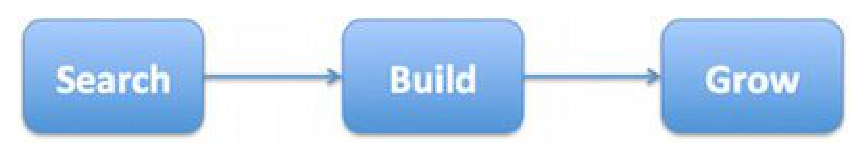
\includegraphics[width=11cm,angle=0]{figuras/ciclo_de_vida_steve_blank02}
\caption{Representação do Ciclo de Vida de uma Startup por \cite{Blank2015}}
\label{Rotulo}
\end{figure}

No primeiro nível, o objetivo da Startup é identificar e validar um modelo de negócios que seja repetível e escalável, em outras palavras: descobrir o que você vai construir e quem vai compra-lo. \citeonline{Blank2014} diz que é normal que sejam necessárias várias iterações e ``pivotagens'' até encontrar um bom produto e um mercado que possa ser atacado. Nesse nível, as Startups costumam ser pequenas e não muito estruturadas, elas ainda estão imersas em um ambiente de extrema incerteza e um cenário de tentativas e erros e por esse motivo é onde a maior parte morre. Na Figura XX \citeonline{Byers2014} apresenta um modelo de como combinar os interesses e paixões dos empreendedores com suas capacidades e oportunidades do mercado com o objetivo de encontrar o ``pote de ouro'', encontrar o que será o seu produto.

\begin{figure}[!htb]
\centering
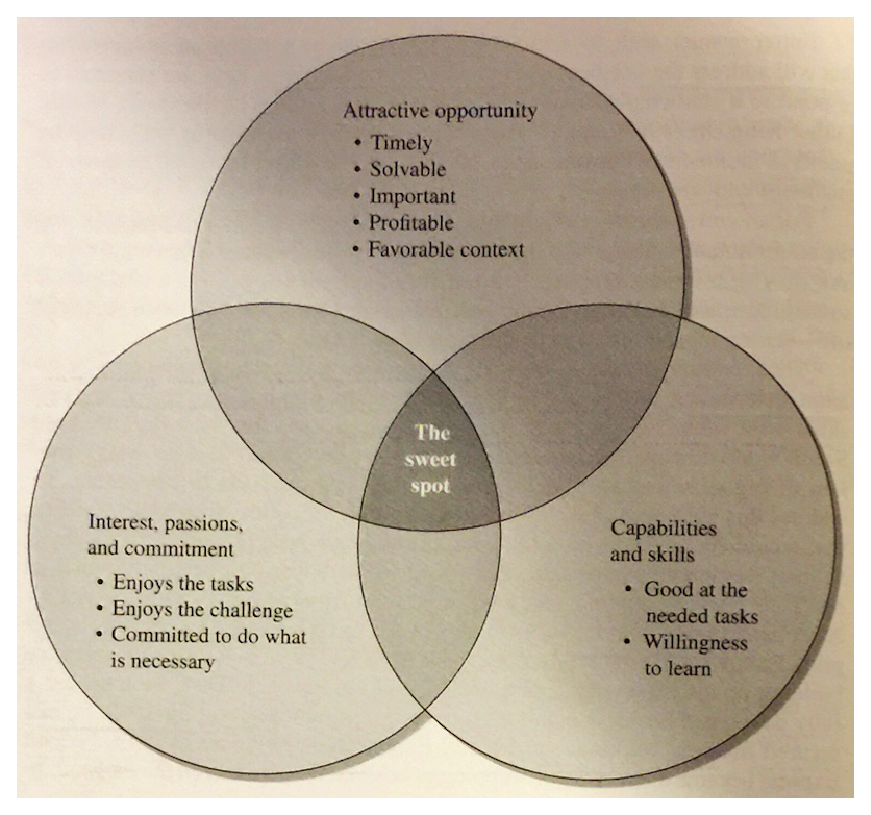
\includegraphics[width=11cm,angle=0]{figuras/the_sweet_spot_byers}
\caption{Representação de como encontrar uma oportunidade por \cite{Byers2014}}
\label{Rotulo}
\end{figure}

Durante o segundo nível, a Startup se encontra em uma fase de transição para se tornar uma empresa que precisa escalar e crescer de forma sustentável. O maior objetivo aqui é atingir um fluxo de caixa positivo, geralmente nesse nível a Startup começa a se tornar uma grande organização, com muitos funcionários, e processos e hierarquias precisam começar a ser definidos para evitar o caos, o crescimento desordenado e garantir que a cultura da empresa será mantida. Segundo Blank, há casos em que as Startups possam ter até 700 funcionários e ainda estarem nesse nível.

No terceiro e último nível, a empresa já atingiu líquidez e está crescendo com a implementação contínua dos processos que foram definidos no nível anterior. É comum que aqui o capital da empresa já tenha sido aberto ou tenha sido vendida. 

\citeonline{Ries2011}, um dos alunos mais ilustres que Steve Blank já teve, trás grande enfâse para a importância que falhar possui no desenvolvimento da sua Startup, e mais precisamente falhar rápido. Seu ciclo de vida tem como objetivo acelerar o caminho da Startup, seja para o sucesso ou para o completo fracasso, caso a equipe chegue a conclusão de que não são capazes de encontrar um modelo de negócios sustentável e repetível. O quanto antes o Empreendedor encontrar o caminho certo, maiores as chances de sua Startup sobreviver. A raiz desse ciclo está representada na figura XX.

A partir das ideias, ele e Blank defendem que o Empreendedor deve construir um Mínimo Produto Viável(ou MVP, como é conhecido pela abreviação do termo na língua inglesa) que corresponda ao menor, ou mais simples, pedaço de produto para que seja possível que a proposta seja validada e lições sejam aprendidas com base no feedback dos usuários. Em seu livro Ries diz que qualquer trabalho adicional além do que é necessário para que a equipe comece a aprender é desperdício, não importa o quão importantes esses recursos extras possam parecer. Para que o aprendizado seja possível, dados precisam ser coletados e medidos. Afinal, como diz o ditado que alguns atribuem à Peter Drucker: ``O que não pode ser medido não pode ser melhorado''. 

\begin{figure}[!htb]
\centering
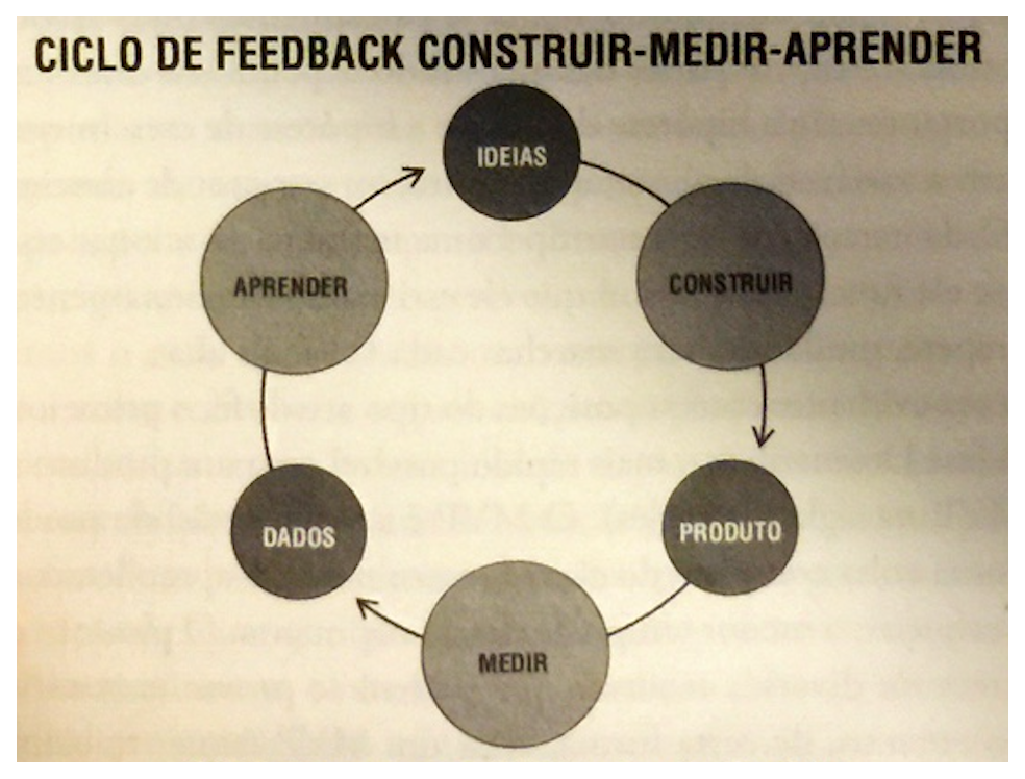
\includegraphics[width=11cm,angle=0]{figuras/ciclo_de_vida_eric_ries}
\caption{Representação do Ciclo de Vida de uma Startup por \cite{Ries2011}}
\label{Rotulo}
\end{figure}

Uma das frases mais emblemáticas do livro ``Startup Enxuta'' é que se empreendedor não pode falhar, então não poderá aprender. E isso se torna claro com esse ciclo de vida proposto por \citeonline{Ries2011}. Quanto maior o número de iterações, maior a quantidade de falhas e consequentemente maior será o aprendizado. Para ele, esse modelo de Costruir, Medir e Aprender com base em loops iterativos e feedbacks constantes

Para \citeonline{Graham2012} o ciclo de vida de uma Startup de sucesso geralmente possui três fases: um período inicial de pequeno ou nenhum crescimento enquanto a Startup ainda está tentando descobrir qual o seu propósito e produto, uma fase intermediária com um rápido crescimento após a descoberta de qual o produto desejado pelas pessoas e como vendê-lo e, por fim, a Startup se torna uma Grande Empresa, cheia de processos e com uma redução da taxa de crescimento, mas um grande domínio do mercado.

\citeonline{Polgar2015} relata que Graham também criou um diagrama da curva de crescimento de uma Startup, representado na Figura XX. Esse ciclo apresenta um momento muito interessante que quase todas as Startups precisam superar: logo após o ápice de entusiasmo e energia dos Empreendedores após ter uma ideia e começar a sua implementação eles encontram a fase que é conhecida como ``Trough of Sorrow'', também referenciado como ``The Chasm'' e o ``Vale da morte'', quando a equipe se depara com a realidade e começa a enfrentar muitas das dificuldades inerentes da criação de uma Startup e de um produto. Também é o momento em que a maior parte irá morrer, como o nome sugere.

\begin{figure}[!htb]
\centering
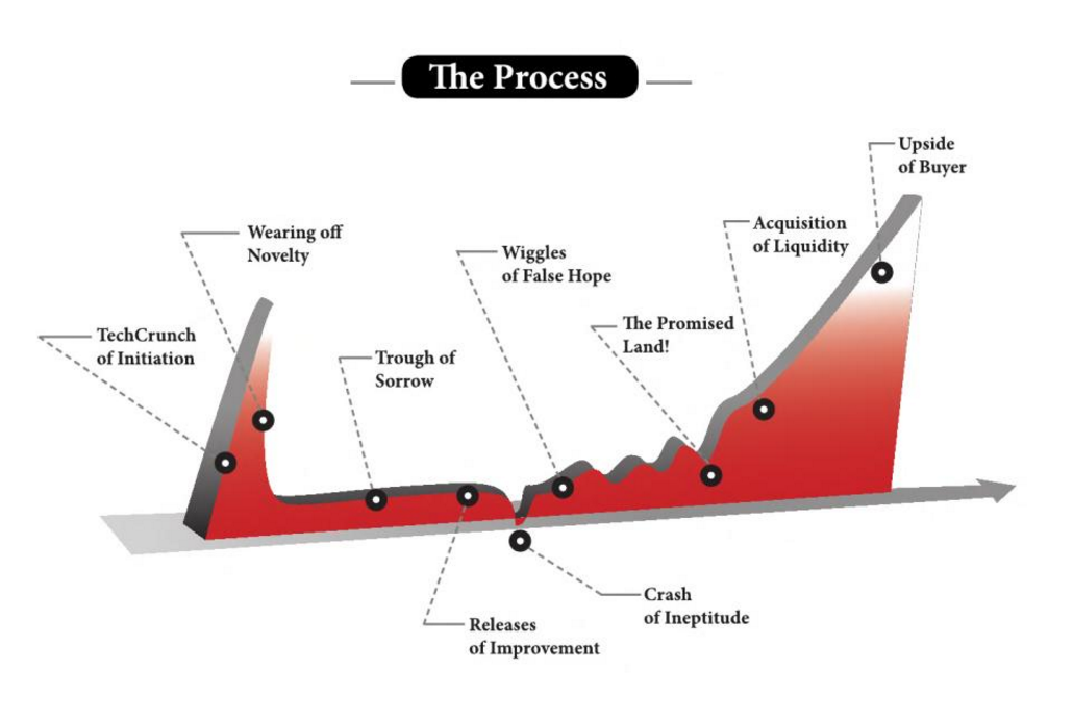
\includegraphics[width=11cm,angle=0]{figuras/startup_curve_by_graham}
\caption{Curva de crescimento de uma Startup por Paul Graham, representado por \cite{Polgar2015}}
\label{Rotulo}
\end{figure}

Essa será uma fase de muita experimentação, falhas, ``pivotagens'' e aprendizados, até que a equipe encontre uma determinada fatia de mercado disposta a comprar seu produto, nesse momento a Startup volta a crescer e começa a escalar. Esse momento está diretamente ligado com a aquisição de clientes, que para muitas Startups seguirá o modelo de penetração de mercado proposto por \citeonline{Moore2014} representado na figura XX.

\begin{figure}[!htb]
\centering
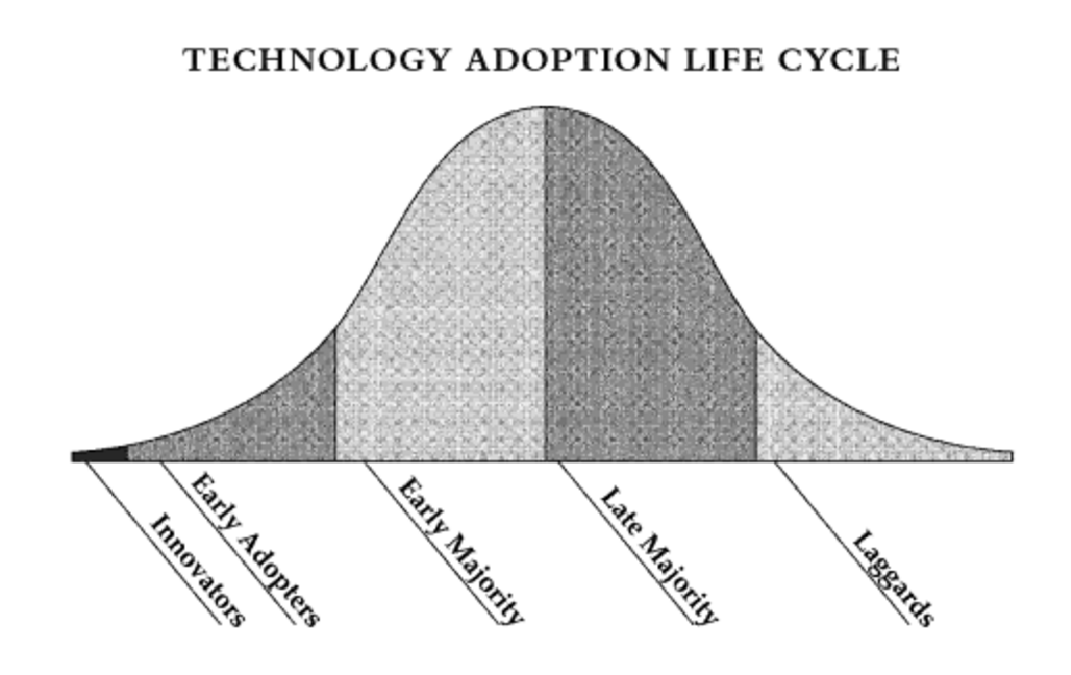
\includegraphics[width=11cm,angle=0]{figuras/chasm_curve}
\caption{Modelo de Penetração de Mercado por \cite{Moore2014}}
\label{Rotulo}
\end{figure}

Quanto maior a fatia do gráfico, maior a quantidade de usuários que estarão consumindo seu produto. Para \citeonline{Moore2014} os Inovadores são aqueles que tem a Tecnologia como uma partes centrais de suas vidas, buscam por produtos inovadores pelo simples prazer de explorar algo novo e estão dispostos a serem usuários antes mesmo do produto ser lançado. 

Os ``Early Adopters'' são muito parecidos com os Inovadores, mas não possuem a Tecnologia como algo tão importante em suas vidas. São apenas usuários com uma grande afinidade com inovações e dispostos a utilizar novas tecnologias e costumam confiar muito na própria intuição antes de testar algum novo produto. 

As próximas fatias do gráfico, referente a grande massa de usuários, irão depender fortemente das impressões dos Inovadores e dos ``Early Adopters'', são eles quem são os influenciadores do mercado e em quem a fatia ``Early Majority'' irá ouvir antes de adquirir um novo produto, que por sua vez serão a base de confiança do grupo ``Late Majority''. Por fim teremos os últimos, os ``Laggards'', que odeiam tecnologia mas eventualmente serão pressionados ou obrigados a adquirirem seu produto. Sem o apoio dos grupos iniciais, segundo Moore, sua Startup nunca superará o Vale da Morte porque todas as fatias são fortemente conectadas e dependentes, mas como um Empreendedor Inovador o seu acesso será apenas a base. Os Inovadores e os ``Early Adopters'' são os dois tipos de usuários críticos que farão o seu produto decolar ou não, e consequentemente sua Startup crescer, escalar e superar o Vale da Morte.

\citeonline{Crowne2002} descreve três fases no ciclo de vida de uma Startup: a primeira, descrita como Startup, a fase de Estabilização e a fase de Crescimento.  A primeira fase é marcada pelo período em que o produto ainda é um conceito até a sua primeira venda concreteizada. A segunda fase acontece até o momento em que o produto e os processos da Startup são estáveis o suficiente para que a entrada de novos clientes não façam a organização perder o controle de si mesmo. A última tem seu início com o começo da venda dos produtos de uma Startup em escala e se mantém até que a Startup alcance o nível de uma organização.

\citeonline{marmer2011startup}, por meio do Startup Genome, organização sem fins lucrativos que realiza análises de Ecossistemas de Startups em todo o mundo entrevistou cerca de 11 mil Empreendedores em 40 Ecossistemas e dividiu o ciclo de vida de uma Startup em seis estágios: a Descoberta, a Validação, a Eficiência, a Escala, a Sustentabilidade e a fase de Conservação. 

Como um dos resultados dessa pesquisa descobriram a grande importância que esse ciclo possui nas chances de sucesso de uma Startup, de forma que aquelas que cresceram de forma muito acelerada e inconsistente, sem respeitar o desenvolvimento de todas as fases do ciclo e suas capacidades, obtiveram resultados muito inferiores, como representado na figura XX. \citeonline{Moore2014} diz que durante o ``Vale da Morte'' é muito importante que a empresa atinga um certo nível de maturidade para conseguir superar essa fase, enfatizando, também, a importância de não pular etapas no desenvolvimento de uma Startup.

\begin{figure}[!htb]
\centering
\includegraphics[width=11cm,angle=0]{figuras/valuation_ao_escalar}
\caption{Representação de como o valor de uma Startup que recebeu investimento mas se desenvolveu de forma consistente cresce muito mais do que o de uma Startup que não respeitou o seu ciclo de vida, por \cite{marmer2011startup}}
\label{Rotulo}
\end{figure}

Também verificaram que cerca de 74\% das Startups que fizeram parte da pesquisa e cresceram de forma prematura falharam, gastaram cerca de 2,3 vezes mais do que a média com aquisição de clientes, nenhuma atingiu a marca de 100 mil usuários, 93\% nunca atingiram 100 mil dólares em vendas mensais e que equipes equilibradas, inclusive com um time de fundadores misto entre profissionais de negócios e profissionais técnicos, receberam investimentos 30\% maiores e tiveram uma taxa de crescimento de base de usuários 3x maior. No artigo citado vários outros indicadores comparativos e fatores que caracterizam um crescimento inconsistente são apresentados. 

\section{O Dinâmico Mercado de Startups e de Investidores}
\label{section:o_dinamico_mercado_das_startups}

Com o advento dos dispositivos móveis e de recursos de internet cada vez mais acessíveis, \citeonline{Paternoster2014} defende que estamos vivendo a Bolha das Startups por conta da grande ploriferação de novas empresas de tecnologia. 

De um lado, dos Empreendedores que conseguem tracionar seus produtos, atrair milhares e até mesmo milhões de usuários e escalar suas empresas, encontramos um mercado agitado e vivendo o seu melhor momento, com milhares de Investidores injetando milhões de dólares nessas Startups acreditando em suas taxas de crescimento fora do convencional, como \citeonline{Graham2012} sugere na casa dos 10\% semanais, e possibilidades de retorno dezenas ou centenas de vezes maiores do que seus investimentos iniciais.

E existem inúmeros casos como esse, como o caso do Investidor Andreessen Horowits, que investiu US\$250 mil no início do Instagram\footciteref{Instagram} e, quando ele foi vendido por US\$1 bilhão para o Facebook\footciteref{Facebook}, lucrou cerca de US\$78 milhões, aproximadamente 312 vezes o que foi investido em apenas dois anos \citeonline{Israel2012, Copelan2012, DailyMail2012}. \citeonline{Sahlman2010} relata que a empresa de investimentos Sequoia Capital\footciteref{Sequoia} faturou 320 vezes o investimentio inicial de US\$12,5 milhões que fez no Google\footciteref{Google} após 7 anos.

A revista americana Fortune fez um levantamento das Startups\footciteref{FortuneStartupRanking} com valor de mercado acima de US\$1 bilhão, conhecidas como Unicórnio, e das dez mais valiosas, todas com valores de mercado acima de US\$11 bilhões, sete foram criadas nos últimos 10 anos, seis foram criadas no estado da Califórnia, nos Estados Unidos da América, e, outras três na China e a restante na Índia.

Porém, do outro lado da moeda, temos dados catastróficos mostrando o quão difícil é criar uma Startup que sobreviva e cresça. Um estudo com 3200 Startups criado por \citeonline{marmer2011startup} verificou que em 3 anos cerca de 92\% quebraram. \citeonline{Blank2014} em seu livro afirma que 90\% dos novos produtos irão falhar. \citeonline{Graham2005}, experiente investidor e empreendedor do Vale do Silício, também menciona em seu blog uma taxa de fracasso entre as Startups gira em torno dos 90\%. 

\citeonline{Crowne2002} mapeou os principais motivos pelos quais Startups falham em três categorias de problemas: na própria Startup, quando o produto começa a se estabilizar no mercado e quando a Startup começa a escalar.

Na primeira categoria, os principais problemas são relativos a inexperiência dos desenvolvedores, falta de gestão de equipe e uma visão fraca do que deve é o produto. Durante a Estabilização os problemas se concentram na falta de controle com o crescimento da Startup, conflitos com novas pessoas, sejam força de trabalho ou investidores, baixa qualidade de produto e muito tempo gasto com requisitos e expectativas mal geridos ou correção de bugs, etc. No Crescimento, mais uma vez a falta de capacidade técnica, de gestão de requisitos e de um bom desenvolvimento de produto são os maiores problemas.

Mas os investidores parecem saber lidar bem com esse cenário, \citeonline{Sahlman2010} relata que cerca de 60\% dos investimentos realizados por empresas de Venture Capital resultam em prejuízo mas que aproximadamente 85\% do faturamento vem de cerca de 12\% dos investimentos que foram feitos em Startups que alcançam um grande sucesso de abertura de capital ou de venda, concretizando lucros acima de 10 vezes o valor de investimento inicial, como representado pela figura XX. 

\begin{figure}[!htb]
\centering
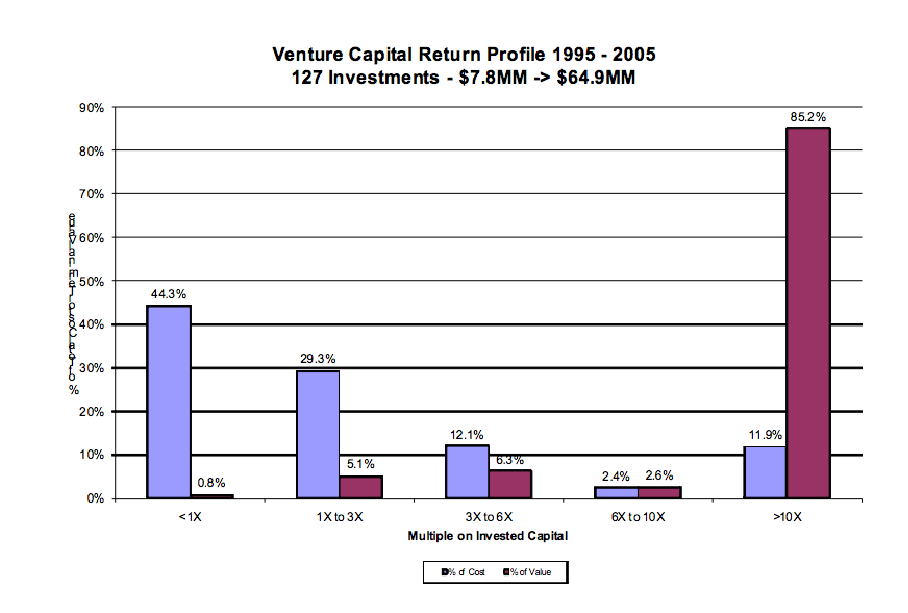
\includegraphics[width=11cm,angle=0]{figuras/venture_capital_profits}
\caption{Relação entre gastos com investimento e retorno de Venture Capital por \cite{Sahlman2010}}
\label{Rotulo}
\end{figure}

Cerca de 300 anos atrás \citeonline{James1953} fez uma análise que demonstra que o valor intríseco de um determinado produto, o seu valor de venda, está associado ao custo de oportunidade e não ao seu custo de produção. Mesmo tantos anos após esse trabalho, é possível fazer uma relação entre esse conceito e o grande valor atribuido à diversas Startups da área de tecnologia, principalmente para aquelas que não geram faturamentos expressivos mas já possuem valor de mercado na casa de milhões, ou bilhões, de dólares, como aconteceu com o Instagram que fora vendido por US\$ 1 bilhão sem faturar 1 centavo sequer, como relatado por \citeonline{Luckerson2013}, ou o WhatsApp que foi comprado por US\$ 19 bilhões faturando cerca de US\$ 20 milhões por ano, conforme relatado por \citeonline{Olson2014}. 

\citeonline{Graham2012} defende que, quando não se pode medir o faturamento da empresa, a melhor opção é usar como métrica de crescimento a quantidade de usuários ativos, visto que quando a solução começar a ser monetizada o faturamento da Startup será uma constante multiplicada por esse número de usuários. Mais uma vez, podemos relacionar uma boa prática moderna com o custo de oportunidade de Cantillon.

\citeonline{Pepper2012} com base na curva do ciclo de vida de uma Startup criada por Paul Graham criou a Curva do Mercado utilizando os mesmos princípios, mas com foco nas tecnologias utilizadas pelo mercado. Essa curva foi representada pela Figura XX.

\begin{figure}[!htb]
\centering
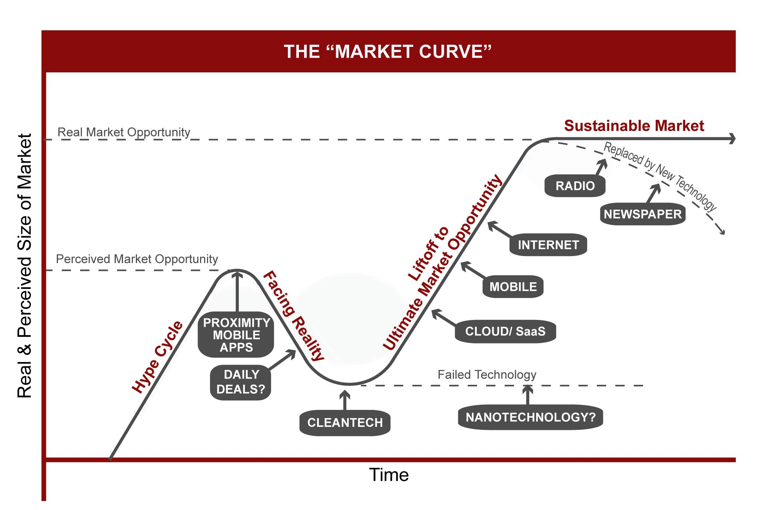
\includegraphics[width=11cm,angle=0]{figuras/market_curve}
\caption{Curva de Mercado de diversas Tecnologias por \cite{Pepper2012}}
\label{Rotulo}
\end{figure}

A primeira fase de crescimento de uma tecnologia, o ``Hiper Ciclo'', surge quando uma oportunidade de mercado é percebida, momento que em 2012 os aplicativos com foco em proximidade e geolocalização, como o Foursquare\footciteref{Foursquare}, estavam em alta, seguido pelo momento em que o mercado se depara com a realidade, chamado de ``Encarando a Realidade'', encontramos a primeira queda, onde citam as empresas de compra coletiva e promoções diárias.

Olhando em retrospecto e de acordo com os índices da NASDAQ\footciteref{NasdaqGroupon}, o mercado de compras coletivas viveu o seu grande momento em meados de 2011, quando cada ação chegou a valer US\$ 26, e justamente em 2012, quando Pepper publicou essa curva de mercado, começou a enfraquecer chegando a casa dos US\$ 2 dólares por ação. Entre 2013 e 2014 houve um novo momento de impulso, com a ação chegando a US\$ 12 mas logo voltou a cair. Atualmente, em 2016, cada ação vale em torno de US\$ 3. Essa curva foi representada na Figura XX.

\begin{figure}[!htb]
\centering
\includegraphics[width=11cm,angle=0]{figuras/stock_market_groupon}
\caption{Valor das ações do Groupon entre 2011 e 2016, retirado do site da NASDAQ}
\label{Rotulo}
\end{figure}

Esse é o momento em que as Tecnologias que falham perdem força e muitas vezes são descartadas por não conseguirem crescer o bastante para a próxima fase. Em seguida, encontramos a ``Decolagem para a Oportunidade de Mercado Final'', quando as novas tecnologias começam a se consolidar, em 2012 a Internet, o modelo de negócios de Software como um Serviço na nuvem e Celulares, até que alcancem na fase do ``Mercado Sustentável'', quando aquela oportunidade de negócio que fora percebida no início se torna uma oportunidade de negócio real. O autor exemplifica sua teoria com um gráfico representando as ações da Amazon\footciteref{Amazon} entre 1998 e 2012 representado pela Figura XX. Vale ressaltar que em 7 de Julho de 2016, de acordo com a NASDAQ, cada ação da Amazon custa US\$ 4876,81, consideralmente mais do que em 2012, quando custava em torno de US\$3000, de acordo com a mesma fonte.

\begin{figure}[!htb]
\centering
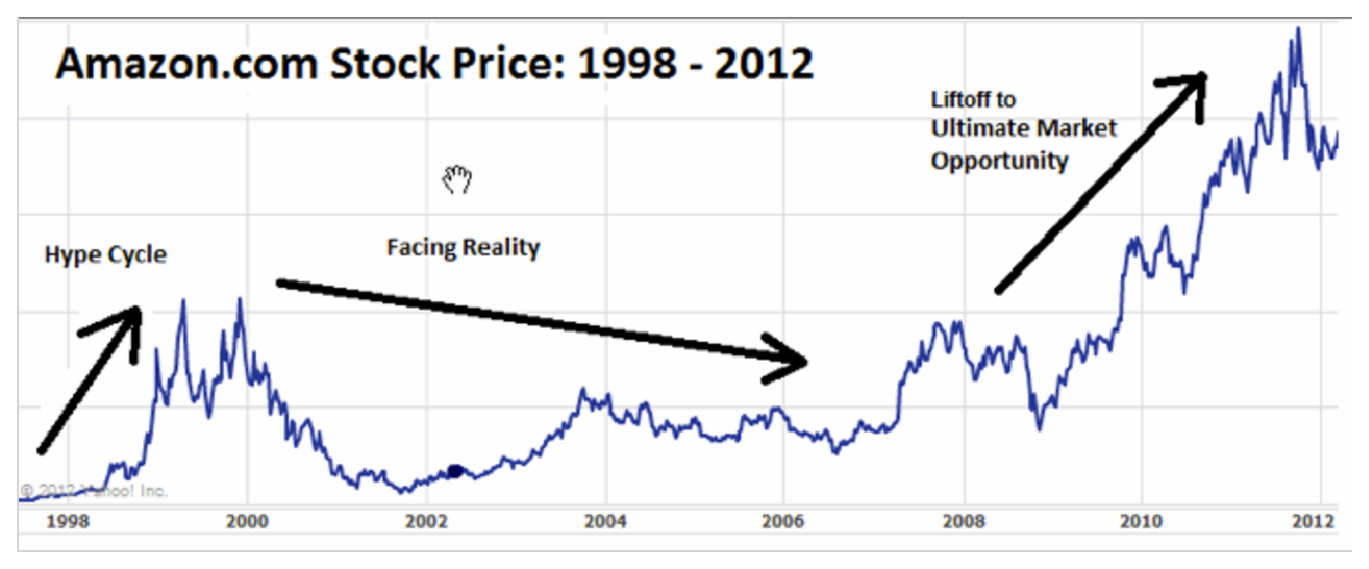
\includegraphics[width=11cm,angle=0]{figuras/stock_market_amazon}
\caption{Valor das ações do Amazon entre 1998 e 2012, criado por \cite{Pepper2012}}
\label{Rotulo}
\end{figure}

\section{O Ecossistema}
\label{section:ecossistemas_e_suas_pecas}

\citeonline{James1953} diz que o crescimento econômico, a formação e o crescimento de cidades está diretamente ligado ao Empreendedorismo e as decisões que são tomadas por Empreendedores. \citeonline{Dalcin2015} relata que alguns dos impactos locais de um bom Ecossistema de Startups envolvem a criação de empregos, o crescimento econômico e a redução da pobreza. 

\citeonline{Schumpeter1934} diz que Empreendedores tendem a se conglomerar em uma mesmo região com o objetivo de obterem benefícios mútuos, criando clusters, que podem ser interpretados como Ecossistemas, e são essenciais para o desenvolvimento local.

\citeonline{Dubini1989} diz que Ecossistemas são marcados pela presença de empresas, uma economia diversificada, uma boa infraestrutura de negócios e investimentos, uma cultura adequada e políticas públicas que apoiem os Empreendedores e a criação de novos empreendimentos. \citeonline{ranga2013triple} trás uma abordagem com o conceito da Hélice Tripla, que representa a interação entre Governo, Indústria e Academia, como representado pela Figura XX. 

\begin{figure}[!htb]
\centering
\includegraphics[width=11cm,angle=0]{figuras/triple_helix}
\caption{Modelo de Hélice Tripla, por \citeonline{ranga2013triple}}
\label{figure:triple_helix}
\end{figure}

\citeonline{isenberg2011introducing} mapeia os Ecossistemas Empreendedores em seis grandes pilares: Política, Finanças, Cultura, Suporte, Capital Humano e Mercado, onde todos devem agir em conjunto para a criação de um Ecossistema saudável e promissor. Essa visão está representada na Figura XX. \citeonline{schwab2015} defende que os pilares são Abertura de Mercados, Capital Humano, Investimento, Apoio do Governo, Ambiente Regulatório, Educação, Universidades e Suporte Cultural.

\begin{figure}[!htb]
\centering
\includegraphics[width=11cm,angle=0]{figuras/isenberg_ecosystem}
\caption{Ecossistemas Empreendedores, por \citeonline{isenberg2011introducing}}
\label{figure:isenberg_ecosystem}
\end{figure}

\citeonline{gumpert1985heart} diz que enquanto o Governo e a Academia podem criar condições favoráveis para que o Empreendedorismo aconteça o envolvimento de indivíduos é essencial, reforçando o modelo criado por Isenberg e indo contra o conceito da Hélice Tripla.

\citeonline{Stangler2015}, por meio da Kauffman Foundation, definem os quatro seguintes indicadores de um Ecossistema vibrante: Densidade, Fluídez, Conectividade e Diversidade. Para o indicador Densidade, eles sugerem que medidas indicadas podem ser a quantidade de novas empresas para cada mil pessoas, a quantidade de emprego nessas empresas e a densidade dos setores, em especial que envolvam alta tecnologia. Para Fluídez indicam o fluxo populacional de uma cidade, a realocação no mercado de trabalho e a quantidade de empresas de alto crescimento. Para se medir Conectividade os dados podem ser relacionados à redes de investidores, conectividade entre programas e a quantidade de spin-offs. Por fim, diversidade idealmente pode ser medida pela quantidade de especializações econômicas, taxa de mobilidade e de imigrantes. O artigo em si não descreve um arcabouço para avaliação de Ecossistemas, mas define bons quatro indicadores que podem ser utilizados por outros trabalhos, por este, inclusive. 

\citeonline{Motoyama2014}, também por intermédio da Kauffman Foundation, identificaram quatro pontos de conexão chave em um Ecossistema Empreendedor e os dividiram em quatro níveis: Conexões entre Empreendedores, Conexões entre Organizações de Suporte, Conexões entre Empreendedores e Organizações de Suporte e Conexões de Suporte Diversas, como eventos. Esses conceitos foram de extrema importância para este Trabalho, visto que é muito claro que são essas Conexões que movem o Ecossistema.

\citeonline{Spigel2015} define Ecossistemas como a união entre elementos culturais, sociais, políticos e econômicos em uma região que propíciam o crescimento de empresas inovadoras e encorajam novos empreendedores e outros atores a assumirem os riscos relacionados a essas empresas. Com um extenso estudo o autor construiu a Tabela XX com os atributos de Ecossistemas Empreendedores, ele também criou uma pirâmide que representa as relações entre esses atributos, representado pela Figura XX.

\begin{table}[!htb]
	\centering
	\label{tabela:attributes_of_entrepreneurship_ecosystems}
	\begin{tabular}{ | p{3cm} | p{4cm} | p{8cm} | }
		\hline
		Tipo & Atributo & Descrição \\ \hline
		Cultura & Apoio & Atitudes culturais que apoiam e transformam atividades empreendedoras, risco e inovação em situações normais. \\ \hline
		Cultura & Histórias de Empreendedorismo & Exemplos locais de empresas e empreendedores de sucesso. \\ \hline
		Social & Talento & Presença de profissionais talentosos e experientes dispostos a trabalhar em startups. \\ \hline
		Social & Investimento & Disponibilidade de capital para investimento de famílias e amigos, investidores anjos e venture capital. \\ \hline
		Social & Redes & Presença de redes sociais que conectem empreendedores, conselheiros, investidores e profissionais que permitam o fluxo livre de conhecimento e experiências. \\ \hline
		Social & Mentores & Empreendedores e profissionais locais bem sucedidos dispostos a contribuir com o crescimento de jovens empreendedores. \\ \hline
		Material & Políticas Públicas & Programas estatais e regulamentações que apoiem o Empreendedorismo ou removam barreiras para a criação de novas empresas. \\ \hline
		Material & Universidades & Universidades e outras instituições educacionais que preparam novos Empreendedores e produzem conhecimento relevante para o Ecossistema. \\ \hline
		Material & Serviços de Suporte & Organizações especializadas em oferecer suporte para novas empresas como advogados, incubadoras, contadores, etc. \\ \hline
		Material & Infraestrutura & Disponibilidade de espaços para escritórios, acesso a recursos de telecomunicação e transporte, etc. \\ \hline
		Material & Abertura de Mercado & Presença de oportunidades locais que permitam que as empresas creçam de forma global. \\ \hline
	\end{tabular}
	\caption{Atributos de Ecossistemas Empreendedores, por \cite{Spigel2015}}
\end{table}

\begin{figure}[!htb]
\centering
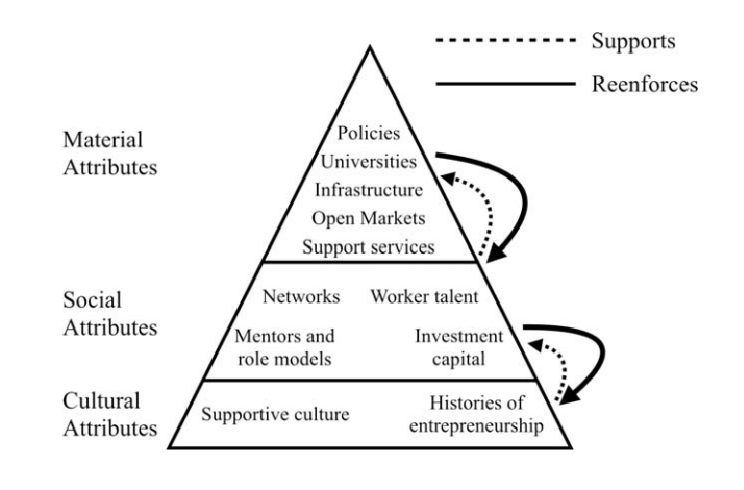
\includegraphics[width=11cm,angle=0]{figuras/relationship_among_ecosystems_attributes}
\caption{Relacionamentos entre atributos de Ecossistemas Empreendedores, por \citeonline{Spigel2015}}
\label{figure:relationship_among_ecosystems_attributes}
\end{figure}

\citeonline{Feld2012}, empreendedor bem sucedido e um especialista em Ecossistemas de Startups, contribuiu a ``Teoria de Boulder'' em que ele define quatro regras para um bom Ecossistema: 1) Precisa ser liderado por Empreendedores; 2) Os líderes precisam assumir um compromisso a longo prazo para com o Ecossistema; 3) O Ecossistema precisa ser inclusivo para qualquer pessoa que queira participar; 4) O Ecossistema precisa ter atividades contínuas que engajem toda a comunidade empreendedora local. Ele também elencou alguns atores que compõem e são de grande importância para Ecossistemas como Empreendedores, Governo, Universidades, Investidores, Mentores, Provedores de Serviço e Grandes Empresas. Outro fator interessante é que ele enxerga Ecossistemas Empreendedores como organismos que estão em constante evolução, e não estruturas bem definidas. Com base nesse princípio ele também faz a divisão de atores entre ``semeadores'' (seeders, aqueles que fomentam e criam o movimento no Ecossistema) e ``alimentadores'' (feeders, todos aqueles que não atuam como semeadores e se beneficiam do crescimento do Ecossistema). 

\citeonline{Stam2015} fez uma ótima síntese dos atributos para um bom Ecossistema que foram explorados no livro ``Startup Communities'' de Feld, exibido pela Tabela XX, e \citeonline{Chua2012} criou um ótimo rascunho sobre o mesmo livro, exibido pela Figura XX.

\begin{table}[!htb]
	\centering
	\label{tabela:attributes_of_entrepreneurship_ecosystems}
	\begin{tabular}{ | p{3cm} | p{12cm} | }
		\hline
		Atributo & Descrição \\ \hline
		Liderança & Grupo forte de empreendedores que são bem conhecidos no Ecossistema, acessíveis e compromissados com o desenvolvimento local da região. \\ \hline
		Intermediários & Mentores e conselheiros bem respeitados que contribuam com o Ecossistema, aceleradoras e incubadoras também podem tomar esse papel. \\ \hline
		Densidade da Rede & Uma comunidade de empreendedores bem sucedidos e muito bem conectados com investidores, mentores, conselheiros, apoiadores, etc. Todos devem estar dispostos a dar mais do que receber do Ecossistema. \\ \hline
		Governo & \\ Forte apoio do governo tanto em ajudar como em entender o contexto das Startups e em como alterar o ambiente regulatório de forma a contribuir com o desenvolvimento de mais empresas. \\ \hline
		Talentos & \\ Diversas opções de talentos com diferentes níveis de experiência e conhecimento disponíveis no mercado local para empresas de todos os tamanhos e estágios em todas as áreas do conhecimento. Boa parte desses profissionais vem da universidade e por isso devem estar bem conectadas com o Ecossistema. \\ \hline
		Apoiadores & \\ Advogados, contadores, etc integrados, acessíveis, efetivos e com uma oferta de serviços com preços adequados. \\ \hline
		Engajamento & \\ Um grande número de eventos para que Empreendedores e Ecossistema se conectem. Podem ser meetups, dias de pitch, hackathons, startup weekends, etc.
		Empresas & \\ Grandes empresas estabelecidas podem ter um grande papel como apoiadores das novas Startups, seja fornecendo infraestrutura, conhecimento ou investimento que os Empreendedores possam utilizar. \\ \hline
		Capital & \\ Uma comunidade forte, apoiadora e presente de investidores dos mais diversos tipos como anjos, venture capital, etc. \\ \hline
	\end{tabular}
	\caption{Atributos de um Ecossistema de Startups bem sucedido, por \cite{Stam2015} e \cite{Feld2012}}
\end{table}

\begin{figure}[!htb]
\centering
\includegraphics[width=11cm,angle=0]{figuras/startup_communities}
\caption{Rascunho, criado por \citeonline{Chua2012}, sobre o livro ``Startup Communities'', criado por {Feld2012}}
\label{figure:startup_communities}
\end{figure}